\francais

\chapter*{Conclusion}

\setcounter{chapter}{4}

\hypertarget{vers-une-meilleure-compruxe9hension-des-dynamiques-forestiuxe8res-en-ruxe9ponse-aux-changements-globaux}{%
\section{Vers une meilleure compréhension des dynamiques forestières en
réponse aux changements
globaux}\label{vers-une-meilleure-compruxe9hension-des-dynamiques-forestiuxe8res-en-ruxe9ponse-aux-changements-globaux}}

De nombreuses études utilisent les données d'inventaire forestier pour
tenter de prédire l'avenir sous les changements climatiques
\citep{boulanger_climate_2017, chen_modeling_2002, iverson_estimating_2008, meier_climate_2012, perie_dominant_2016, vissault_biogeographie_2016}.
Mais, s'il est possible de faire des prédictions de grands changements
pour 2050, soit dans 30 ans, ne devrait-on pas déjà commencer à
percevoir les premiers signes de ces changements dans les données
cumulées depuis 1970, il y a 50 ans? Quelles informations pouvons-nous
tirer de ces changements récents? Par ailleurs, les projections des
effets du changement climatique sur les forêts ont généralement mis
l'accent sur la capacité des espèces à tolérer les augmentations de
température et les sécheresses et à se disperser, mais ils ont rarement
intégré les effets des perturbations. Étant donné l'importance des
perturbations naturelles et de celles générées par l'exploitation
forestière dans la dynamique des forêts \citep{turner_disturbance_2010},
ces projections du futur basées seulement sur le changement climatique
sont-elles réalistes ou trompeuses? Si les perturbations interagissent
avec le changement climatique et exacerbent la mortalité des arbres, les
nouvelles politiques d'aménagement du territoire et de la forêt qui
reposent sur des modèles incomplets risquent d'être mal adaptées.

À travers ma thèse de recherche, j'ai tenté d'apporter des éléments de
réponses à ces questionnements. Ses trois chapitres ont permis de
d'analyser en détail les multiples aspects de la dynamique des forêts au
cours des dernières décennies afin de mieux comprendre la réponse aux
effets combinés du changement climatique et des perturbations. Dans
l'ensemble, mes résultats soulignent le rôle central des perturbations
dans la réponse des forêts face au changement climatique. En effet, la
composition et la structure (Chapitre \ref{chap1}), la dynamique de
transition (Chapitre \ref{chap2}), ainsi que la dynamique de
régénération (Chapitre \ref{chap3}) des forêts de l'écotone
boréal-tempéré au Québec sont principalement contrôlées par les
perturbations et leurs effets semblent interagir avec ceux des
changements climatiques. J'ai montré comment les perturbations
accélèrent la réponse des communautés forestières aux changements
climatiques, révélant des synergies qui ont le potentiel de modifier
l'avenir de nos forêts.

\hypertarget{ruxe9organisation-des-communautuxe9s}{%
\subsection{Réorganisation des
communautés}\label{ruxe9organisation-des-communautuxe9s}}

Dans le chapitre \ref{chap1}, je me suis intéressée aux moteurs des
changements de composition dans les communautés forestières. Au cours
des dernières décennies, les perturbations (par exemple, les coupes à
blanc, les épidémies d'insectes, les incendies) ont été les principaux
facteurs de changement de composition des communautés forestières,
i.e.~la diversité \(\beta\) temporelle, dans l'écotone tempéré-boréal.
En revanche, les effets uniques du changement climatique sur la
diversité \(\beta\) temporelle sont très faibles. Sans approfondir, on
aurait pu conclure prématurément que le changement climatique n'a pas
influencé la composition des forêts au cours des dernières décennies.
L'analyse des changements des traits écologiques de la communauté a
permis de révéler un phénomène de thermophilisation des forêts à travers
le Québec, i.e. une augmentation des espèces de climat chaud au
détriment des espèces de climat froid. En outre, la thermophilisation a
été plus grande et s'est étendue plus au nord dans les communautés
modérément perturbées que dans celles qui n'ont pas été perturbées ou
qui ont subi des perturbations majeures.

Les résultats de ce chapitre ont soulevé d'autres questions importantes:
la thermophilisation récentes des forêts indique-t-elle un changement
permanent ou bien seulement une dynamique transitoire? Et, si les
perturbations modérées favorisent la thermophilisation, est-ce qu'elles
pourraient accélérer des changements d'état permanents? C'est la
question que j'ai creusée dans le second chapitre de ma thèse.

\hypertarget{la-dynamique-des-foruxeats}{%
\subsection{La dynamique des forêts}\label{la-dynamique-des-foruxeats}}

Dans le chapitre \ref{chap2}, j'ai analysé la dynamique de transition
des forêts du Québec en utilisant un modèle à quatre états, soit boréal,
mixte, tempéré et pionnier. Encore une fois, les perturbations
naturelles et anthropiques ressortent comme les moteurs principaux de la
dynamique de transition des forêts au cours des dernières décennies.
Alors que les perturbations majeures déclenchent surtout des transitions
vers l'état pionnier, les perturbations modérées favorisent les
transitions de l'état mixte vers l'état tempéré. De plus, les
perturbations modérées accélèrent le taux de renouvellement des forêts
et, à long terme, favorisent une augmentation de la proportion de forêts
tempérées dans le paysage. Par conséquent, les perturbations modérées
ont le potentiel de catalyser un déplacement plus rapide de l'écotone
boréal-tempéré vers le nord sous l'effet du changement climatique.
Toutefois, contrairement à mes attentes, les transitions des forêts
mixtes à tempérées ne découlaient pas d'une hausse du recrutement
d'arbres tempérés mais plutôt des processus de mortalité et de
croissance.

Si les transitions reposent davantage sur la mortalité et que celle-ci
n'est pas équilibrée par le recrutement de nouveaux arbres, les forêts
mixtes pourraient en fin de compte dépérir. Alors que les perturbations
modérées favorisent la thermophilisation des forêts et la transition de
peuplements mixtes à tempérés, comment influencent-elles le recrutement
des espèces tempérées? Les analyses rapportées dans les deux premiers
chapitres étant basées sur les arbres matures seulement, elles ne
pouvaient pas bien répondre à cette nouvelle question. Il fallait donc
analyser la dynamique des jeunes arbres (i.e.~les gaulis).

\hypertarget{la-ruxe9guxe9nuxe9ration-des-foruxeats-les-premiers-pas-de-la-migration}{%
\subsection{La régénération des forêts: les premiers pas de la
migration}\label{la-ruxe9guxe9nuxe9ration-des-foruxeats-les-premiers-pas-de-la-migration}}

Dans le chapitre \ref{chap3}, j'ai d'abord mis en lumière de grands
déplacements de distribution vers le nord pour les gaulis (i.e., jeunes
arbres entre 1 et 9 cm de diamètre) de l'érable rouge, l'érable à sucre
et le bouleau jaune dans les forêts non perturbées. Toutefois, sous
l'influence des perturbations modérées, seuls les érables ont migré et
aucune espèce ne s'est déplacée sous l'influence des perturbations
majeures. En revanche, la répartition du hêtre à grandes feuilles n'a
pas bougé dans tous les cas. Ces résultats soulignent que les futurs
déplacements d'aire de répartition des espèces peuvent dépendre de leur
réponse aux perturbations. De plus, il y a une légère tendance au
déplacement des gaulis vers le bas des pentes, surtout dans les régions
proches de leur limite nord. Ces tendances pourraient signaler le début
d'une migration des populations marginales vivant au sommet des
collines. Mes résultats ont montré que, malgré l'effet positif des
coupes partielles sur le recrutement, la prévalence des contraintes
locales associées à la composition des peuplements et aux conditions
topo-édaphiques risque de freiner la migration des espèces tempérées
vers le nord.

\hypertarget{des-foruxeats-en-transformation-des-individus-aux-biomes}{%
\section{Des forêts en transformation: des individus aux
biomes}\label{des-foruxeats-en-transformation-des-individus-aux-biomes}}

Les effets des changements environnementaux se répercutent à chaque
niveau d'organisation de la biodiversité, se transmettant des individus
jusqu'au biome, en passant par les populations, les communautés et les
écosystèmes \citep{bellard_impacts_2012, parmesan_globally_2003}. En
effet, conformément aux concepts de la science des systèmes complexes,
les changements démographiques au bas de la hiérarchie peuvent faire
émerger, par des processus d'organisation autonome, des réorganisations
massives à l'échelle régionale \citep[Fig.
\ref{fig4.2};][]{filotas_viewing_2014, messier_managing_2013}. Les
résultats de ma thèse permettent de bien illustrer ces processus
ascendants et en interaction par lesquels les forêts de l'écotone
boréal-tempéré sont en train de se transformer. L'interprétation de mes
résultats sous la perspective des systèmes complexes permet de mieux
comprendre la réponse des forêts sous l'effet combiné du changement
climatique et des perturbations ainsi que les conséquences écologiques
qui en découlent.

\newpage

\begin{figure}
\centering
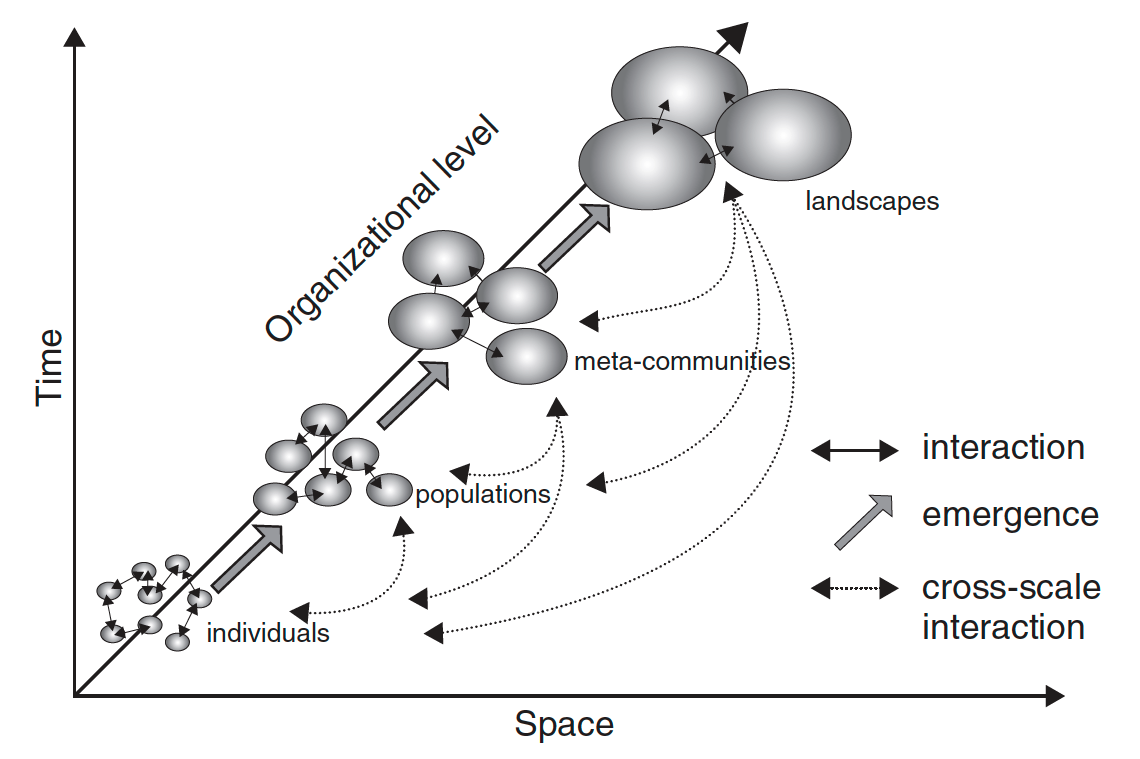
\includegraphics[width=.8\textwidth]{conclusion/figures/complex.png}
\caption[Effets des changements environnementaux sur les différents niveaux d'organisation de la biodiversité]{Représentation conceptuelle des effets des changements environnementaux sur les forêts sous l'angle d'un système complexe. Les changements dans la dynamique des forêts sont transférés de façon ascendante entre les différents niveaux d'organisation de la biodiversité. Des interactions et des rétroactions ont lieu entre les entités à l'intérieur et à travers les échelles spatiales, temporelles et hiérarchiques. Les entités qui interagissent à un niveau donnent naissance à des entités émergentes de niveau supérieur, dont l'existence, à son tour, affecte le comportement des entités de niveau inférieur. Schéma tiré de Messier \emph{et al.} (2013).}
\label{fig4.2}
\end{figure}

\hypertarget{changements-duxe9mographiques}{%
\subsection{Changements
démographiques}\label{changements-duxe9mographiques}}

Dans un premier temps, le réchauffement climatique favorise le
recrutement, la survie et la croissance des espèces tempérées à leur
limite nord
\citep{boisvertmarsh_divergent_2019, bolte_understory_2014, fisichelli_temperate_2014, goldblum_tree_2005, grundmann_impact_2011},
ce qui leur confère un avantage compétitif par rapport aux espèces
boréales. Mais, en l'absence de perturbations, les arbres poussent
lentement, leurs taux de mortalité et de recrutement sont faibles et la
compétition pour l'espace et la lumière est intense.

Des perturbations peuvent cependant éliminer les individus des espèces
résidentes. Dans la zone d'étude, les perturbations naturelles et
anthropiques ont provoqué une mortalité disproportionnée d'une espèce
dominante dans les forêts mixtes (Chapitre \ref{chap2}). En effet, le
sapin baumier a subi une mortalité massive suite aux grandes épidémies
de tordeuse des bourgeons de l'épinette dans les années 1967-1992
\citep{duchesne_population_2008}. De plus, cette espèce est aussi la
plus coupée au Québec. Suite à une perturbation modérée (p. ex.,
épidémie légère, coupe partielle), les trouées dans la canopée résultant
de la perte de cette espèce boréale ubiquiste et abondante ont
probablement permis de réduire la compétition et de libérer des
ressources, favorisant ensuite la croissance rapide des espèces
tempérées compagnes, telles que les érables rouge et à sucre ainsi que
le bouleau jaune (Chapitre \ref{chap2}). De plus, alors que les
perturbations naturelles semblent avoir un effet plutôt délétère, les
coupes partielles favorisent une hausse du recrutement de ces espèces
tempérées à leur limite nord (Chapitre \ref{chap3}). En cas de
perturbations majeures (p.~ex., grand feu, coupe totale), la majorité
des arbres en place meurent ce qui crée des ouvertures de très grande
superficie. Ces paysages nouvellement ouverts sont colonisés rapidement
par des espèces pionnières telles que le peuplier faux-tremble et le
bouleau blanc (Chapitre \ref{chap2}) qui peuvent disperser leurs graines
sur de longues distances et croître rapidement en conditions lumineuses
\citep{boucher_fire_2017, grondin_have_2018}. Suite à une perturbation
majeure, les espèces tempérées peuvent être plus lentes à revenir parce
qu'elles se dispersent sur des distances plus courtes
\citep{scheller_spatially_2005}.

\hypertarget{dynamique-des-populations}{%
\subsection{Dynamique des populations}\label{dynamique-des-populations}}

Le réchauffement et les perturbations peuvent donc exercer leur
influence sur la dynamique des populations des espèces par le biais de
plusieurs processus démographiques, notamment la reproduction, le
recrutement, la croissance et la mortalité. Ces changements à l'échelle
des individus et des sites s'accumulent dans le temps et dans l'espace
pour altérer l'abondance et l'aire de répartition des populations
\citep{holt_theoretical_2005}. Lorsque les effets sur les individus
d'une espèce sont généralement négatifs, le taux de croissance de la
population diminu; certaines populations pourraient être amenées à
disparaître localement et, dans le pire des cas, régionalement. À
l'inverse, lorsque les effets sur les taux démographiques d'une espèce
sont positifs, le taux de croissance de la population augmente, ce qui
peut entraîner une augmentation locale de l'abondance et une expansion
régionale de l'aire de répartition.

Ces effets sur les taux démographiques des espèces ne sont pas
aléatoires, mais sont déterminés par leurs tolérances physiologiques,
leurs stratégies d'histoire de vie et leurs capacités de dispersion
\citep{aubin_traits_2016, estrada_species_2015}. La diversité des
caractéristiques écologiques spécifiques est sans doute à l'origine de
la grande variabilité dans les réponses des arbres face aux multiples
stresseurs environnementaux \citep{serra-diaz_disturbance_2015}. Alors
que le réchauffement peut favoriser le taux de croissance des
populations d'espèces qui sont limitées par les températures très
froides, les perturbations devraient promouvoir les espèces
opportunistes, intolérantes à l'ombre, avec une bonne capacité de
dispersion et de reproduction végétative \citep[Chapitre
\ref{chap3};][]{danneyrolles_stronger_2019, de_frenne_microclimate_2013}.
Par exemple, l'érable rouge, dont la distribution au nord est en partie
limitée par un faible niveau de reproduction sexuée
\citep{tremblay_potential_2002}, est reconnue comme une espèce
super-généraliste et opportuniste, capable de coloniser rapidement des
sites variés après une perturbation
\citep{abrams_red_1998, fei_rapid_2009}. Ces caractéristiques pourraient
donc expliquer l'expansion rapide qu'a connue l'érable rouge au Québec
sous l'effet combiné du réchauffement et des perturbations (Chapitres
\ref{chap1}, \ref{chap2} et \ref{chap3}). En revanche, certaines espèces
limitées par la dispersion comme le tilleul d'Amérique, ou limitées à un
habitat spécifique comme l'érable argenté, ou encore intolérantes aux
perturbations comme la pruche du Canada, pourraient ne pas profiter des
opportunités de recrutement et de croissance suivant des perturbations,
et ce même si le climat est devenu plus favorable pour ces espèces.

La sensibilité au climat peut varier entre les différents processus
démographiques \citep{niinemets_responses_2010}. Par exemple, comme la
régénération est souvent plus sensible que la survie des adultes aux
stress hydrique ou thermique \citep{niinemets_responses_2010}, une
population peut persister pendant des décennies ou des siècles sur un
site donné, même si les conditions climatiques sont devenues
défavorables à sa régénération \citep{talluto_extinction_2017}. Pour
cette raison, \citet{jump_altitude-for-latitude_2009} ont suggéré que
l'expansion à la limite nord de la distribution d'une espèce sera plus
rapide que les changements à la limite sud puisque la reproduction et le
recrutement sont plus sensibles aux changements environnementaux que la
mortalité des individus établis. Dans les forêts du Québec, les données
montrent effectivement une augmentation rapide de l'abondance (Chapitre
\ref{chap1}) et du recrutement des espèces tempérées dominantes
(Chapitre \ref{chap3}). Toutefois, la perte des espèces boréales a sans
doute été tout aussi importante sinon plus puisque la mortalité n'était
pas contrôlée par un stress climatique mais surtout par des
perturbations directes comme les coupes, les feux et les épidémies
(Chapitres \ref{chap1} et \ref{chap2}). Ainsi, contrairement à
l'hypothèse avancée par \citet{jump_altitude-for-latitude_2009}, les
perturbations risquent d'accélérer la contraction de l'aire de
répartition des espèces boréales, tandis que l'effet sur l'expansion des
espèces tempérées à leur limite nord pourrait être beaucoup plus lent en
raison des contraintes au recrutement (Chapitre \ref{chap3}). En effet,
le recrutement des espèces tempérées est largement dépendant de la
présence des arbres matures conspécifiques pour la dispersion et est
freiné par la compétition des espèces boréales de même que par les
conditions de mauvais drainage (sites hydriques) dans les bas de pente
(Chapitre \ref{chap3}).

\hypertarget{dynamique-des-communautuxe9s}{%
\subsection{Dynamique des
communautés}\label{dynamique-des-communautuxe9s}}

Les changements démographiques des espèces se traduisent donc, à
l'échelle locale, en pertes et en gains d'espèces qui influencent la
composition et la structure des communautés forestières. Dans l'écotone
boréal-tempéré, la thermophilisation des forêts résultait principalement
du gain d'une seule espèce tempérée, l'érable rouge, combiné à la perte
de deux espèce boréales dominantes, le sapin et l'épinette noire, et ce
phénomène était accentué par les perturbations modérées (Chapitre
\ref{chap1}). Ainsi, sans perturbation, le renouvellement de la
communauté est très lent, tandis que celui-ci est accéléré par les
perturbations modérées (Chapitres \ref{chap1}, \ref{chap2} et
\ref{chap3}). En revanche, les perturbations majeures détruisent la
communauté en place et réinitialisent la succession à partir du début,
ce qui entraîne surtout des gains en espèces pionnières (Chapitres
\ref{chap1} et \ref{chap2}). Au cours de ma thèse, j'ai pu montrer
comment ces changements de composition résultent de l'action conjointe
de trois mécanismes démographiques qui altèrent la trajectoire de
succession après une perturbation modérée: (1) la mortalité d'une espèce
dominante; (2) le relâchement de la croissance des adultes des espèces
tempérées compagnes; et (3) le recrutement accru des gaulis des espèces
tempérées compagnes ou présentes dans le voisinage.

Les conséquences au niveau des communautés des changements d'aires de
répartition spécifiques aux espèces pourraient mener à la formation de
communautés sans analogues, i.e.~des communautés dans lesquelles
coexistent des espèces dans des combinaisons historiquement rares ou
inconnues \citep{williams_novel_2007}. Les modèles de distribution
d'espèces sous l'effet du changement climatique prédisent un grand
potentiel d'augmentation de la richesse au Québec
\citep{berteaux_changements_2014}. Toutefois, mes résultats soulignent
que seule une poignée d'espèces tempérées prospèrent sous ce nouveau
régime de perturbations anthropiques. Par conséquent, il est fort
probable que les forêts de l'écotone boréal-tempéré ne connaîtront pas
un enrichissement, mais plutôt un appauvrissement associé à l'expansion
d'une ou de quelques espèces. On prévoit en outre que le déclin des
espèces boréales actuellement dominantes, soit le sapin et l'épinette,
risque de s'accentuer dans les prochaines décennies dans les domaines de
la sapinière en raison du réchauffement climatique
\citep{dorangeville_beneficial_2018}. Le remplacement de ces espèces
résineuses par des espèces feuillues pourrait avoir des conséquences
économiques importantes. Par exemple, l'expansion de l'érable rouge
pourrait compromettre l'approvisionnement en espèces résineuses à grande
valeur commerciale dans la forêt mixte. Les pratiques sylvicoles devront
être révisées pour s'adapter à la nouvelle réalité puisqu'elles ont été
élaborées en fonction de la composition et de la dynamique naturelle des
forêts et dépendent de la régénération naturelle
\citep{pinna_amenagement_2009}.

\hypertarget{duxe9placement-des-grands-biomes-forestiers}{%
\subsection{Déplacement des grands biomes
forestiers}\label{duxe9placement-des-grands-biomes-forestiers}}

Les effets cumulés des changements à l'échelle des individus, des
populations et des communautés peuvent entraîner un déplacement des
grands biomes forestiers à l'échelle régionale, notamment une expansion
de la forêt tempérée au détriment de la forêt mixte (Chapitre
\ref{chap2}). Cette réorganisation régionale de la composition des
forêts peut interagir avec le fonctionnement des écosystèmes à l'échelle
locale et les processus à l'échelle globale \citep[\emph{cross-scale
interactions};][]{peters_crossscale_2007}. Ces changements de
fonctionnement à l'écotone risquent d'être d'autant plus grands puisque
les espèces feuillues et les espèces résineuses présentent des
différences importantes sur le plan de leurs caractéristiques et
fonctions écologiques \citep{wardle_terrestrial_2011}. L'enfeuillement
des forêts mixtes pourrait par exemple influencer localement la qualité
de la litière, le taux de décomposition de la matière organique et la
composition des microorganismes du sol
\citep{laganiere_how_2010, legare_influence_2005}. Les changements dans
la composition, la structure d'abondance et la distribution spatiale des
forêts affecteront également la survie et la distribution des nombreuses
espèces de mammifères, d'oiseaux et d'insectes qui en dépendent pour
s'abriter et se nourrir \citep{friggens_effects_2018}. Comme les espèces
feuillues sont moins inflammables et moins sensibles aux insectes
ravageurs que les conifères, leur augmentation dans le paysage forestier
peut modifier le régime régional de perturbations
\citep{terrier_potential_2013, mffp_insectes_2018}. À long terme,
l'expansion du biome tempéré au détriment des forêts mixtes et boréales
pourrait avoir un effet sur le climat global en augmentant la
séquestration du carbone \citep{thurner_carbon_2014} et l'albédo
\citep{anderson_biophysical_2011}.

\hypertarget{les-perturbations-catalyseurs-de-changements-dans-les-foruxeats}{%
\section{Les perturbations --- catalyseurs de changements dans les
forêts}\label{les-perturbations-catalyseurs-de-changements-dans-les-foruxeats}}

Les effets combinés du changement climatique et des perturbations
peuvent donner naissance à des dynamiques non-linéaires conduisant à un
changement de régime écologique \citep[\emph{regime shift}; Fig.
\ref{fig4.2};][]{harris_biological_2018, scheffer_catastrophic_2001}. Un
changement de régime résulte d'une réorganisation rapide de la
composition et de la structure d'un écosystème qui entraîne un
basculement vers un nouvel état alternatif stable
\citep{scheffer_catastrophic_2001}. Par exemple, si la transition des
forêts mixtes vers des forêts à dominance tempérée documentée dans le
Chapitre \ref{chap2} persiste, cette transformation pourrait bel et bien
s'avérer être un changement de régime.

En théorie, des changements d'état stable peuvent subvenir suivant deux
mécanismes: (1) des changements graduels dans les conditions
environnementales jusqu'à un niveau critique où le système s'effondre
soudainement, et (2) des perturbations trop sévères ou en rafale qui
poussent le système hors de son bassin d'attraction
\citep{scheffer_catastrophic_2001}. Par exemple, la grande augmentation
des taux de mortalité des arbres dans l'ouest des États-Unis en réponse
à un stress hydrique grandissant \citep{van_mantgem_apparent_2007}
pourrait être le signe avant-coureur d'un dépérissement massif des
forêts. Dans un autre cas, \citet{payette_shift_2003} ont montré que les
impacts cumulés de la coupe forestière, suivie d'une épidémie d'insectes
puis d'un incendie, pourraient avoir des effets catastrophiques sur la
régénération des arbres, entraînant la transition d'une pessière dense
en un milieu ouvert dominé par le lichen. Bien que les deux mécanismes
puissent indépendamment mener à une transition rapide d'état, leurs
effets synergiques augmentent le risque de changements rapides de régime
écologique \citep{harris_biological_2018, scheffer_catastrophic_2001}.
Mes résultats supportent cette hypothèse et suggèrent que les forêts
répondent à l'effet cumulé d'un stress à long terme causé par le
changement climatique (i.e., \emph{press disturbance}), en combinaison
avec des événements de mortalité aigus \citep[i.e., \emph{pulse
disturbance};][]{jentsch_theory_2019, harris_biological_2018}. Ainsi, le
réchauffement climatique érode la résilience des forêts mixtes tandis
que les perturbations éliminent les espèces boréales en place et
accélèrent le processus de succession vers davantage d'espèces tempérées
adaptées aux températures plus chaudes (Chapitres \ref{chap1},
\ref{chap2} et \ref{chap3}).

\hypertarget{ruxe9silience-uxe9tats-alternatifs-stables-et-changement-de-ruxe9gime}{%
\subsection{Résilience, états alternatifs stables et changement de
régime}\label{ruxe9silience-uxe9tats-alternatifs-stables-et-changement-de-ruxe9gime}}

Les résultats issus de ma thèse m'ont amenée à réfléchir en profondeur à
la dynamique de changement de régime écologique dans le contexte de
l'écotone boréal-tempéré et à redéfinir le paysage conceptuel des états
stables de cette région (Fig. \ref{fig4.1}). Le long du gradient
latitudinal, la forêt boréale au nord et la forêt tempérée au sud sont
les seuls états stables possibles (Fig. \ref{fig4.1}a). Ces états
forestiers ont une grande résilience face aux perturbations de type
\emph{pulse} qui sont dans la plage de variabilité naturelle de leur
région \citep{grondin_have_2018}; une perturbation naturelle ou
anthropique peut déplacer le système à l'intérieur du bassin
d'attraction, mais le système peut ensuite se rétablir et revenir à son
état initial.

Dans la zone de transition entre ces deux grands biomes, on trouve la
forêt mixte, un état relativement rare qui change facilement d'un état
de dominance à l'autre (Fig. \ref{fig4.1}a). Ceci suggère que la forêt
mixte ne serait pas l'état stable de la région, mais que cette
communauté représente plutôt un état instable où le système n'est que
transitoire. La coexistence des espèces boréales, tempérées et
pionnières dans la forêt mixte est maintenue grâce à l'hétérogénéité des
perturbations naturelles combinée à des différences dans les stratégies
de cycle de vie des espèces
\citep{bouchard_tree_2006, kneeshaw_natural_2007} sous un climat donné.

En plus des perturbations de type \emph{pulse}, le climat global change
graduellement et de façon persistante, ce qui peut altérer la forme du
paysage des états stables (Fig. \ref{fig4.1}b). À mesure que le climat
se réchauffe, les forêts peuvent perdre leur capacité à se rétablir
puisque les espèces en place ne sont plus aussi bien adaptées au climat
\citep{johnstone_changing_2016}. Mon interprétation est que le
réchauffement modifie surtout le bassin d'attraction de l'état mixte et
abaisse le seuil critique à franchir pour se rendre à l'état tempéré
(Fig. \ref{fig4.1}b). De plus, le réchauffement peut rendre le bassin de
l'état tempéré plus large et profond, donc plus attractif, et,
inversement, celui de l'état boréal moins profond. Ces modifications de
la courbe des états alternatifs stables fragilisent la forêt mixte,
mais, en l'absence de perturbation, la grande inertie des forêts cache
la perte de résilience de l'état mixte. Parce qu'ils ont une longue
durée de vie, les arbres peuvent faire paraître les forêts inébranlables
face aux changements environnementaux alors même que la niche de
régénération est en train de se déplacer
\citep{boisvertmarsh_divergent_2019, sittaro_tree_2017}. Toutefois, une
perturbation peut facilement faire basculer le système vers un nouvel
état; la composition des forêts mixtes peut donc se déplacer rapidement
vers une dominance en espèces tempérées qui sont mieux adaptées aux
températures plus chaudes.

\newpage

\begin{figure}
\centering
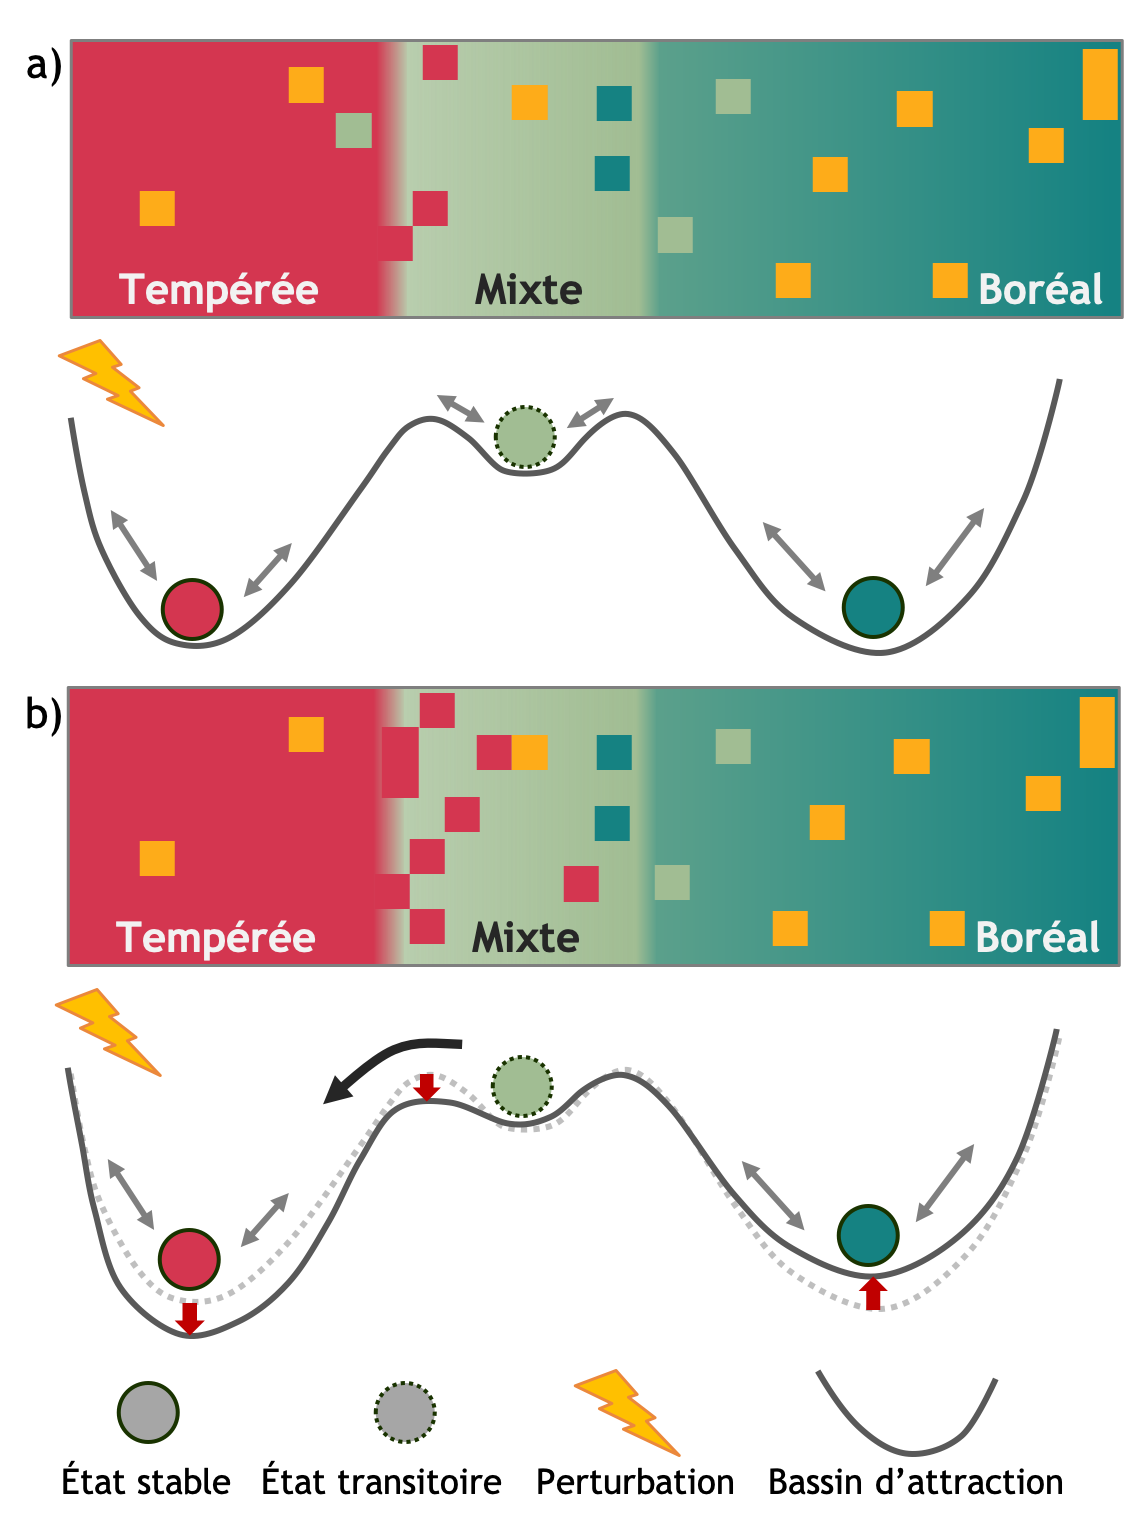
\includegraphics[width=.63\textwidth]{conclusion/figures/etat_alternatif2.png}
\caption[États alternatifs stables le long du gradient latitudinal]{Nouvelle représentation conceptuelle des états alternatifs stables le long du gradient latitudinal (a) sans changement climatique et (b) avec changement climatique. Dans ce schéma, la bille caractérise l'état de l'écosystème à un instant donné, le long de la courbe; les vallées sont les bassins d'attraction des équilibres stables et les sommets des collines sont les équilibres instables. Le schéma rectangulaire représente le paysage correspondant. Au sud du gradient latitudinal de température, un seul état stable existe, la forêt tempérée (en rouge). Au nord du gradient, l'état stable dominant est la forêt boréale (en turquoise). Ce sont des états stables dynamiques; les perturbations peuvent faire déplacer la boule dans son bassin d'attraction et elle peut même passer par l'état pionnier (un état transitoire non représenté le long de la courbe, mais représenté par des carrés jaunes dans le paysage). La forêt étant habituellement résiliente aux perturbations, elle retourne ensuite vers son état initial. Au centre, dans l'écotone, la forêt mixte (en vert) serait un état transitoire entre les deux états stables dominants; cet état peut être maintenu grâce à la dynamique naturelle des perturbations. Dans le panneau (b), le changement du climat peut provoquer un changement de la forme du paysage de différentes façons: (1) en abaissant le seuil pour passer de l'état mixte à tempéré, (2) en creusant et en élargissant le bassin d'attraction de l'état tempéré et (3) en rendant moins profond le bassin d'attraction de l'état boréal. Ces modifications font en sorte que la bille dégringole plus souvent de la vallée mixte vers la vallée tempérée sous l'effet d'une perturbation.}
\label{fig4.1}
\end{figure}

Contrairement aux perturbations modérées, les perturbations majeures
détruisent toutes la communauté en place et poussent le système vers
l'état pionnier, i.e. des peuplements dominés par des espèces
intolérantes à l'ombre ou bien avec pas ou très peu d'arbres (Chapitre
\ref{chap2}). Leur effet à long terme est difficile à prévoir à partir
des données d'inventaire puisque les systèmes n'ont sans doute pas eu le
temps de revenir à un état stable dans la période couverte par cette
étude (1970 à 2018). En effet, l'état pionnier est en général un état
transitoire. Il est donc fort probable que la majorité des forêts soient
encore en train de se déplacer vers leur état d'équilibre. Toutefois, il
se pourrait que certaines forêts se soient transformées définitivement.
Par exemple, les peuplements de peuplier faux-tremble dans les pessières
noires représentent normalement un état de transition, mais, sous
l'effet des coupes forestières, ces peuplements sont en expansion et
semblent se maintenir \citep{grondin_les_2003}. Pour évaluer la
trajectoire des forêts sévérèment perturbées, il faudra attendre encore
quelques années.

La fréquence et la sévérité des perturbations naturelles, telles que les
incendies, les épidémies d'insectes, les sécheresses et les vagues de
chaleur, devraient augmenter dans de nombreuses régions du monde
\citep{bergeron_past_2006, seidl_forest_2017}. À la lumière de mes
résultats, cela pourrait conduire à des changements majeurs dans la
composition des forêts au cours des prochaines décennies et
potentiellement à des modifications permanentes des états forestiers.
Cependant, si les perturbations deviennent trop fréquentes et trop
intenses, les forêts pourraient basculer vers une dominance en espèces
pionnières de début de succession. Des comportements non-linéaires dans
les réponses des écosystèmes forestiers impliquent que de nombreuses
projections sous-estiment probablement l'ampleur des changements futurs
de la biodiversité \citep{scheffer_catastrophic_2001}. Une telle
conclusion souligne l'importance de tenir compte de l'effet synergique
des perturbations et du changement climatique dans les stratégies de
gestion forestière ainsi que dans les modèles de prédiction.

\hypertarget{lamuxe9nagement-forestier-dans-un-monde-en-changement-et-incertain}{%
\section{L'aménagement forestier dans un monde en changement et
incertain}\label{lamuxe9nagement-forestier-dans-un-monde-en-changement-et-incertain}}

Les effets multiples des changements globaux sur la dynamique forestière
soulèvent un défi majeur pour l'aménagement de nos forêts. Face à la
rapidité et à l'incertitude de ces changements, nos pratiques visant à
contrôler et à prédire précisément l'évolution de nos forêts risquent
d'être contre-productive \citep{puettmann_critique_2009}. Étant donné
que les coupes forestières ont une influence majeure sur la composition
(Chapitre \ref{chap1}), la dynamique (Chapitre \ref{chap2}) et la
régénération des forêts (Chapitre \ref{chap3}) et interagissent avec le
changement du climat, il est évident que les futures politiques
d'aménagement auront un rôle fondamental à jouer pour maintenir ou
développer la capcité des forêts à s'adapter rapidement face aux
changements globaux.

Le réchauffement que nous avons connu jusqu'à présent n'est que mineur
par rapport aux projections faites pour la fin du siècle
\citep{ipcc_climate_2014}. Néanmoins, tel que mis en évidence dans
l'ensemble de ma thèse, de grandes transformations sont déjà évidentes à
toutes les échelles de l'organisation écologique. Avec l'accélération
des changements environnementaux et l'inertie inhérente de la dynamique
forestière, le déséquilibre ne pourra que s'accentuer et les réponses
des forêts dépendront des dynamiques transitoires déjà en cours. En ce
moment au Québec, l'estimation de la productivité des peuplements
forestiers repose sur des taux de mortalité et de croissance prévisibles
sous un climat constant. En aménagement forestier, on simplifie et on
présume que le climat est stable et que les forêts sont à l'équilibre. À
court terme, ces hypothèses sont valables, alors qu'à long terme elles
sont particulièrement problématiques dans le contexte du changement
climatique. En effet, comme la dynamique forestière n'est pas à
l'équilibre \citep{talluto_extinction_2017}, la trajectoire de
succession et la niche de régénération sont facilement altérées sous
l'effet combiné du réchauffement et des perturbations (Chapitres
\ref{chap2} et \ref{chap3}). Les prédictions issues de calculs qui
supposent l'équilibre pourraient à la fois sur-estimer la capacité de
régénération et de croissance de certaines espèces et sous-estimer la
mortalité associée à des extrêmes climatiques, menant ainsi à une
planification mal adaptée. Par conséquent, les activités de gestion
doivent non seulement anticiper le changement, mais aussi reconnaître
que les systèmes actuels ont déjà été transformés et sont en train de se
transformer davantage. L'importance de ce point a été bien exprimée par
\citet{seastedt_management_2008} :

\begin{quote}
In managing novel ecosystems, the point is not to think outside the box
but to recognize that the box has moved, and in the 21st century, the
box will continue to move more rapidly.
\end{quote}

\hypertarget{uxe9volution-des-concepts-damuxe9nagement-forestier-au-quuxe9bec}{%
\subsection{Évolution des concepts d'aménagement forestier au
Québec}\label{uxe9volution-des-concepts-damuxe9nagement-forestier-au-quuxe9bec}}

Une importante volonté de gestion durable des forêts s'est développée
dans les dernières décennies à travers le monde. Jusqu'à la fin du
XX\textsuperscript{e} siècle, les modèles de gestion étaient basés une
vision utililariste de la forêt et étaient centrés sur la production de
bois \citep{kuuluvainen_natural_2012}. Depuis les années 1990, la
foresterie a évolué vers un objectif d'aménagement qui intègre davantage
de critères écologiques et sociaux \citep{messier_managing_2013}. Au
Québec, dans la foulée du documentaire \emph{L'erreur boréale} de
Richard Desjardins et Robert Monderie, sorti en 1999, une grande
réflexion s'est amorcée sur l'exploitation de la forêt publique. Pour
répondre aux inquiétudes de la population, la Commission d'étude sur la
gestion de la forêt publique québécoise fut formée en 2003 et a déposé
en 2004 un rapport qui faisait état de la situation et formulait de
nombreuses recommandations pour améliorer et moderniser la gestion des
forêts
\citep{commission_detude_sur_la_gestion_de_la_foret_publique_quebecoise_commission_2004}.
En réponse à ces recommandations, le Québec s'est doté de la Loi sur
l'aménagement durable du territoire forestier, en vigueur depuis 2013,
qui promeut un aménagement écosystémique. L'aménagement écosystémique
s'inspire des patrons spatio-temporels générés par les perturbations
naturelles, qui servent d'états de référence, afin de maintenir les
écosystèmes dans leur plage de variabilité naturelle historique et ainsi
réduire les écarts entre les forêts naturelles et aménagées
\citep{attiwill_disturbance_1994, vaillancourt_implementation_2009}.

L'aménagement écosystémique représente une grande avancée car il intègre
un ensemble d'objectifs sociaux et écologiques plus larges et reconnaît
l'importance de la biodiversité et des processus écologiques qui
influencent la dynamique forestière
\citep{kuuluvainen_forest_2009, messier_functional_2019}. Cette nouvelle
approche de gestion présente néanmoins une lacune majeure: ces pratiques
de gestion ne sont pas conçues pour faire face au rythme rapide des
changements globaux et à l'incertitude croissante qui en découle
\citep{messier_dealing_2016, millar_climate_2007}. En effet, des
pratiques de gestion qui visent à maintenir la composition et la
structure des forêts historiques de référence vont devenir de plus en
plus difficiles à mettre en \oe{}uvre
\citep{boulanger_climate_2019, duveneck_measuring_2016} et ne permettent
pas nécessairement d'améliorer la capacité des écosystèmes à s'adapter à
un nouvel ensemble de conditions environnementales
\citep{seastedt_management_2008}. Bien que le retour vers des conditions
de référence historiques deviendra sans doute insoutenable dans le
futur, les informations historiques documentant la dynamique naturelle
des écosystèmes forestiers seront essentielles pour mieux appréhender
les dynamiques du futur \citep{harris_ecological_2006}.

\hypertarget{perspective-amuxe9nager-les-foruxeats-pour-augmenter-leur-ruxe9silience-et-leur-capacituxe9-adaptative}{%
\subsection{Perspective: aménager les forêts pour augmenter leur
résilience et leur capacité
adaptative}\label{perspective-amuxe9nager-les-foruxeats-pour-augmenter-leur-ruxe9silience-et-leur-capacituxe9-adaptative}}

La solution privilégiée pour faire face au changement climatique est
d'accroître la résilience et la capacité adaptative des forêts
\citep{messier_managing_2013, seastedt_management_2008}. Alors que la
résilience permet à une forêt de retrouver sa structure et ses fonctions
d'origine, la capacité adaptative lui permet de diverger d'un état
antérieur qui était mal adapté aux conditions environnementales
\citep{filotas_viewing_2014}. Les perturbations naturelles et les
variations climatiques sont inévitables mais en développant une grande
diversité, les forêts auront la possibilité de se réorganiser et de
s'adapter à des conditions climatiques sans analogues
\citep{messier_dealing_2016}. S'appuyant sur l'hypothèse d'assurance
\citep[de l'anglais \emph{insurance
hypothesis};][]{yachi_biodiversity_1999}, l'idée est de favoriser la
diversité génétique, spécifique, fonctionnelle et structurale dans les
forêts afin d'augmenter les chances que certaines espèces continueront à
assurer principaux services écosystémiques même si d'autres
disparaissent.

Pour favoriser la capacité adaptative des forêts, il faut avant tout
maintenir la diversité naturelle que l'on trouve à toutes les échelles
spatiales, du peuplement jusqu'au biome, de manière à conserver les
options d'adaptation qui existent déjà. Par exemple, bien que peu
résilientes, les forêts mixtes du Québec ont montré une bonne capacité
adaptative face au changement climatique puisqu'elles ont réussi à se
réorganiser de manière à ajuster leur composition aux nouvelles
conditions environnementales. En effet, suite à une perturbation, des
trajectoires diversifiées peuvent émerger dans les peuplements mixtes
puisqu'ils présentent une hétérogénéité en termes de structure, d'âge,
de tolérance physiologique et de stratégies d'histoire de vie.

Dans d'autres cas, il sera peut-être nécessaire de cultiver activement
la capacité adaptative des écosystèmes grâce à l'aménagement. Ce
principe pourrait devenir important dans les forêts boréales étant donné
leur composition très homogène et leur très grande inertie face au
changement climatique. En effet, alors qu'il y a eu très peu de
transitions vers l'état mixte et pas de thermophilisation des
communautés, on a plutôt observé une dynamique de remplacement entre les
états pionnier et boréal (Chapitres \ref{chap1} et \ref{chap2}). Comme
les forêts du nord du Québec sont très pauvres en espèces, étant
largement dominées par l'épinette noire et le sapin baumier, elles ont
moins de ressources que les forêts mixtes pour faire face aux
changements récents et futurs, ce qui pourrait limiter leur capacité à
s'ajuster et à s'éloigner d'un état parfois mal adapté. De plus, selon
les scénarios d'émissions de gaz à effet de serre élevés, le climat de
la forêt boréale de l'est de l'Amérique du Nord devrait ressembler à
celui de la forêt tempérée d'ici la fin du siècle
\citep{gauthier_boreal_2015}. Toutefois, la migration des espèces
tempérées dans ces régions semble limitée par plusieurs facteurs
non-climatiques, notamment leur capacité de dispersion, la compétition
par les espèces boréales, ainsi que les conditions édaphiques
\citep[Chapitre
\ref{chap3};][]{carteron_soil_2020, solarik_priority_2019}. Des
plantations d'enrichissement pourraient alors s'avérer nécessaires pour
faciliter la migration des espèces tempérées vers le nord et assurer la
résilience des forêts \citep{duveneck_measuring_2016}. Par exemple, et
comme cela a été suggéré pour la migration postglaciaire des arbres
\citep{mclachlan_molecular_2005}, les populations aujourd'hui marginales
pourraient jouer un rôle très important dans la migration future des
arbres en réponse au changement climatique (Chapitre \ref{chap3}).
Ainsi, la création d'îlots de forêts mixtes sur les sommets de collines
dans les forêts boréales assurerait la présence de semenciers de
différentes espèces capables de coloniser rapidement les sites après
perturbation lorsque les conditions climatiques seront adéquates.
Finalement, étant donné les interactions entre échelles, les changements
de régime écologique, la variabilité des réponses des espèces ainsi que
l'importance des événements stochastiques dans la trajectoire des
forêts, il devient de plus en plus clair qu'on ne peut forcer un
peuplement à se développer dans une direction prédéterminée précise en
fonction de nos besoins en bois \citep{puettmann_critique_2009}. Des
recherches récentes encouragent donc à revoir la planification de façon
à avoir des objectifs plus larges et plus flexibles qui permettent un
ensemble de différentes trajectoires futures à l'échelle régionale
\citep{messier_dealing_2016, puettmann_critique_2009}.

L'idée de favoriser la diversité pour assurer la résilience est déjà
prise en compte dans l'aménagement écosystémique et constitue donc une
porte d'entrée au concept d'adaptation au changement climatique
\citep{samuel_foret_2011}. Toutefois, il faut éviter de mettre tous nos
\oe{}ufs dans le même panier. Les projections climatiques nous ont
informé d'un risque croissant de vagues de chaleur et de sécheresse
\citep{ipcc_climate_2014}. Par conséquent, il apparaît logique de mettre
l'accent sur la promotion des espèces qui résistent à la sécheresse.
Mais, dans un contexte d'incertitude, cette stratégie ne suffit pas
puisqu'il est possible que ce ne soit pas la sécheresse qui causera le
plus grand stress aux forêts, mais plutôt l'augmentation de la fréquence
des feux, l'arrivée de nouveaux insectes ravageurs ou encore les
variations des températures printanières. De plus, comme je l'ai montré
dans cette thèse, tous ces facteurs de risque peuvent interagir entre
eux et mener à des changements rapides et inattendus des écosystèmes
forestiers. La grande incertitude associée aux prédictions des effets
attendus des changements climatiques doit être intégrée dans la gestion
forestière de façon à prendre en compte un large éventail de
vulnérabilités des arbres \citep{messier_dealing_2016}. Pour permettre à
l'écosystème de résister ou de s'adapter à ces multiples facteurs de
stress, on pourrait profiter des coupes à rétention variable ou des
plantations pour promouvoir les mélanges d'espèces, définies en fonction
du domaine bioclimatique, ayant des caractéristiques fonctionnelles
diverses, allant des tolérances physiologiques (aux feux, aux ravageurs,
à la sécheresse), aux différents modes de régénération \citep[p.~ex.,
banque de graines, cônes sérotineux, reproduction
végétative;][]{messier_functional_2019, puettmann_critique_2009}.

\hypertarget{au-deluxe0-des-foruxeats-aplanir-la-courbe-du-changement-climatique}{%
\section{Au-delà des forêts --- Aplanir la courbe du changement
climatique}\label{au-deluxe0-des-foruxeats-aplanir-la-courbe-du-changement-climatique}}

Au cours des dernières décennies, l'ouest du Canada a subi une épidémie
sans précédent de dendroctone du pin ponderosa, une grave sécheresse
(2001--2003) et des saisons de feux extrêmes. Les effets synergiques de
ces perturbations ont entraîné un dépérissement rapide et extensif des
forêts \citep{williamson_climate_2009}. De telles catastrophes
naturelles en rafales montrent que la capacité des gouvernements à
s'adapter et à contrôler les dommages peut rapidement être excédée. Or,
les prédictions annoncent une accélération de la fréquence et de la
sévérité des événements climatiques extrêmes \citep{ipcc_climate_2014}.
Si nous n'agissons pas maintenant pour décarboniser notre économie et
changer la trajectoire dangereuse dans laquelle nous sommes engagés, le
climat mondial continuera de se dérégler et la multiplication des
événements climatiques extrêmes dépassera la capacité des systèmes
naturels et humains à se rétablir après les perturbations
\citep{ipcc_summary_2018}. Ainsi, sans mesures d'atténuation du
changement climatique, les stratégies d'aménagement visant à augmenter
la résilience et la capacité adaptative des écosystèmes risquent de
s'avérer vaines. Le récent rapport spécial du GIEC a conclu que limiter
le réchauffement climatique à 1.5 \(^{\circ}\)C est possible mais
exigera des transitions rapides et radicales dans tous les aspects de la
société \citep{ipcc_summary_2018}.

Au cours des premiers mois de 2020, la planète entière a fait face à la
pandémie de la COVID-19 et les gouvernements ont adopté des mesures
draconiennes pour tenter d'en atténuer les conséquences. Le message a
été clair: il fallait ralentir le rythme de propagation de la maladie
pour ``aplanir la courbe'' et éviter de dépasser la capacité des
hôpitaux à traiter les malades. Ce même concept s'applique également à
la crise climatique: limiter le réchauffement climatique permettrait de
ne pas dépasser la capacité de support de la Terre et donnerait aux
sociétés et aux écosystèmes une plus grande marge de man\oe{}uvre pour
s'adapter. La réponse des gouvernements et de la population à la
pandémie de la COVID-19 nous a montré que nous pouvons agir rapidement
et mettre la santé des individus devant celle de l'économie. Cette crise
sanitaire souligne également qu'il serait préférable d'adopter des
mesures préventives afin d'atténuer le changement climatique plutôt que
d'attendre passivement de frapper un mur et d'être forcé à vivre dans
l'état d'urgence. Maintenant que nous comprenons mieux les conséquences
de l'inaction, la priorité est d'utiliser l'ensemble de nos
connaissances scientifiques pour construire un scénario positif et
durable pour l'avenir \citep{bennett_bright_2016}. Ainsi, comme l'a
écrit Antoine de Saint-Exupéry
\citeyearpar{saint-exupery_citadelle_1948} dans Citadelle:

\begin{quote}
Pour ce qui est de l'avenir, il ne s'agit pas de le prévoir, mais de le
rendre possible.
\end{quote}
